\subsection{Configuration}
\vspace{1cm}

Dans un premier temps, afin de faciliter la configuration de l’accès à la base de données lors de la mise en production, j’ai mis en place un fichier de configuration général \colored{globals.php}.\\
Ce fichier contenait un panel de variables de configuration différentes en fonction de l’environnement (développement ou production).

\vspace{1cm}

\begin{figure}[!h]
    \centering
    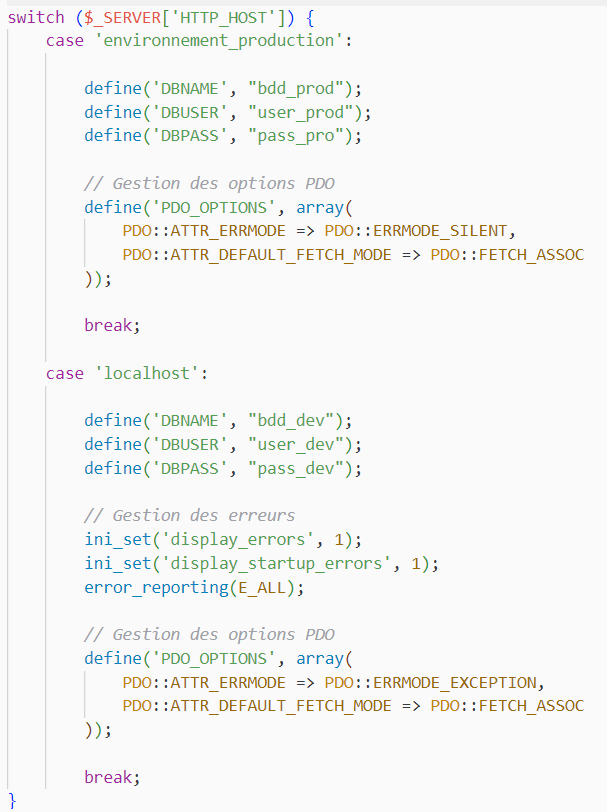
\includegraphics[height=15cm]{globals_code.png}
    \caption{Fichier de configuration d'environnement}
\end{figure}

\newpage

Les paramètres de connexion à la base de données, et l’affichage des erreurs sont différents en fonction de l’environnement : les erreurs sont remontées seulement en environnement de développement.\\ 

Mon tuteur m’a également demandé de la flexibilité pour le nom des tables constituant la base de données, car il risquait d’être amené à modifier certains d’entre eux dans le futur. \\ 

J’ai décidé pour cela d’inclure un fichier \colored{config.json} permettant la modification totale du nom des tables et des colonnes, sans impacter la structure interne de celles-ci.

\begin{figure}[!h]
    \centering
    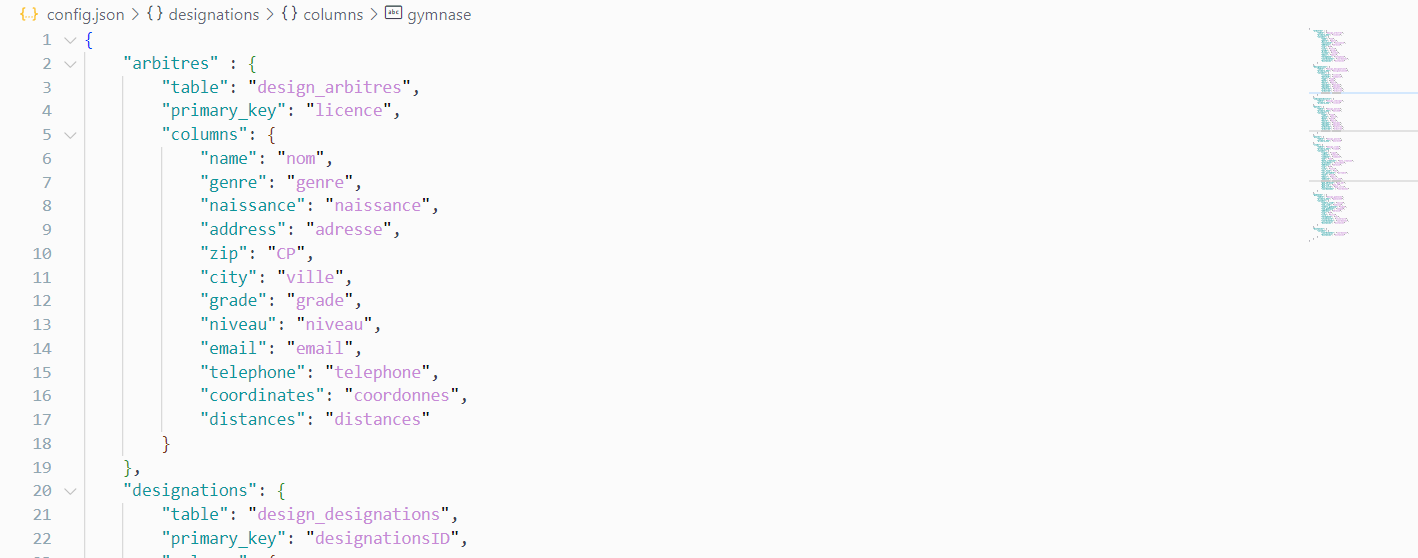
\includegraphics[width=\linewidth]{config.png}
    \caption{Contenu du fichier de configuration du nom des tables}
\end{figure}

\vspace{0.5cm}

Pour récupérer les informations de ce fichier, j’ai également créé un Trait et une méthode associée que je pourrai réutiliser dans mes classes pour récupérer ces informations.

\vspace{1cm}

\begin{figure}[!h]
    \centering
    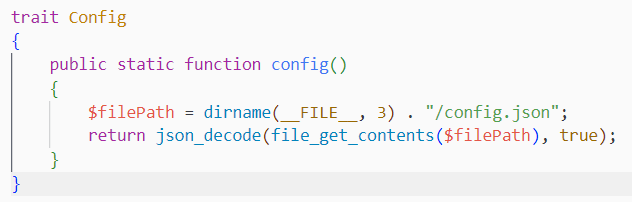
\includegraphics{config_code.png}
    \caption{Trait d'accès au nom des tables dans le fichier de configuration associé}
\end{figure}

\newpage

Ce trait récupère le fichier \colored{config.json} relativement à l’arborescence des dossiers du projet, et renvoi le contenu de celui-ci sous forme de tableau associatif grâce à la fonction \colored{json\_decode()}.

Enfin, dans un but de travailler régulièrement avec la base de données, j’ai mis en place une classe \colored{Database} permettant d’effectuer de façon statique une connexion à celle-ci via une instance de l’objet \textbf{PHP Data Object (PDO)}.

\vspace{2cm}

\begin{figure}[!h]
    \centering
    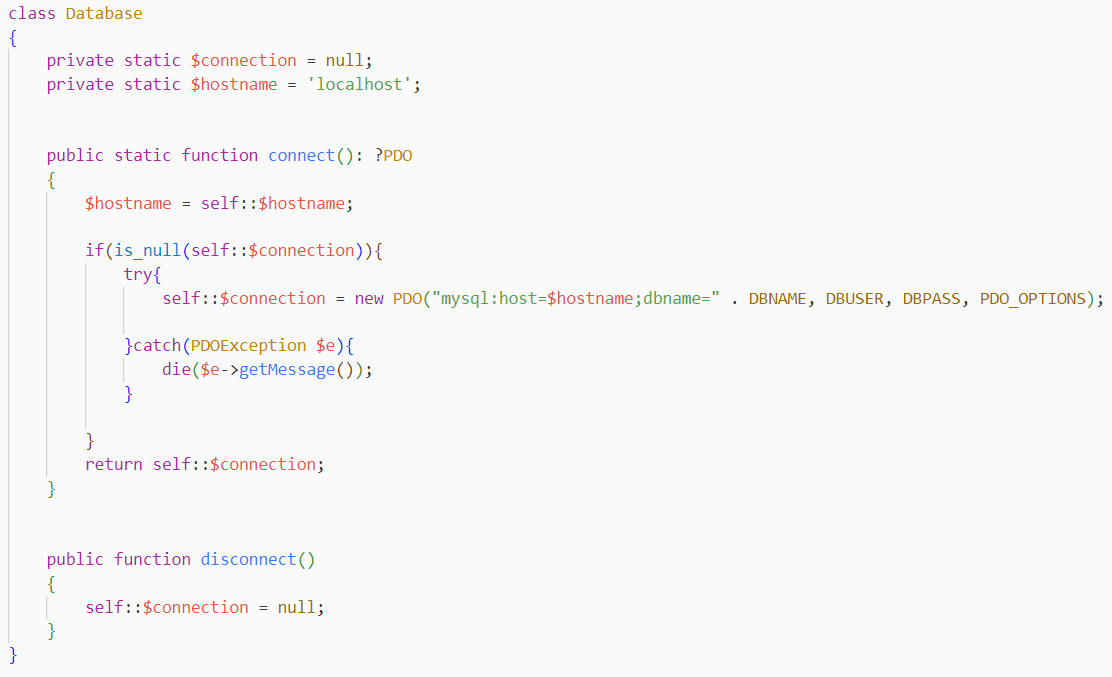
\includegraphics[width=\linewidth]{database_code.png}
    \caption{Composant d'accès à la base de données}
\end{figure}

\newpage
